
\documentclass[letterpaper,hide notes,xcolor={table,svgnames},pdftex,10pt]{beamer}
\def\showexamples{t}

\usecolortheme{crane}
\setbeamertemplate{navigation symbols}{}

\usetheme{MyPittsburgh}
\usepackage{hyperref}
\usepackage{graphicx,xspace}
\usepackage[normalem]{ulem}
\usepackage{multicol}
\usepackage{amsmath,amssymb,amsthm,graphicx,xspace}
\newcommand\SF[1]{$\bigstar$\footnote{SF: #1}}

\usepackage[sfdefault,lf]{carlito}
\usepackage[T1]{fontenc}
\usepackage[scaled]{beramono}
\usepackage{tikzpagenodes}
\newcommand{\Rplus}{\protect\hspace{-.1em}\protect\raisebox{.35ex}{\small{\small\textbf{+}}}}
\newcommand{\Cpp}{\mbox{C\Rplus\Rplus}\xspace}

\newcounter{tmpnumSlide}
\newcounter{tmpnumNote}

\newcommand\mnote[1]{%
	\addtocounter{tmpnumSlide}{1}
	\ifdefined\showcues {~\tiny\fbox{\arabic{tmpnumSlide}}}\fi
	\note{\setlength{\parskip}{1ex}\addtocounter{tmpnumNote}{1}\textbf{\Large \arabic{tmpnumNote}:} {#1\par}}}

\newcommand\mmnote[1]{\note{\setlength{\parskip}{1ex}#1\par}}


\newcommand\mquestion[2]{{~\color{red}\fbox{?}}\note{\setlength{\parskip}{1ex}\par{\Large \textbf{?}} #1} \note{\setlength{\parskip}{1ex}\par{\Large \textbf{A}} #2\par}\ifdefined \presentationonly \pause \fi}

\newcommand\blackboard[1]{%
	\ifdefined   \showblackboard
		{#1}
	\else {\begin{center} \fbox{\colorbox{blue!30}{%
						\begin{minipage}{.95\linewidth}%
							\hspace{\stretch{1}} Some space intentionally left blank; done at the blackboard.%
						\end{minipage}}}\end{center}}%
	\fi%
}

\usepackage{listings}
\lstset{%
	keywordstyle=\bfseries,
	aboveskip=15pt,
	belowskip=15pt,
	captionpos=b,
	identifierstyle=\ttfamily,
	frame=lines,
	numbers=left, basicstyle=\scriptsize, numberstyle=\tiny, stepnumber=0, numbersep=2pt}

\usepackage{siunitx}
\newcommand\sius[1]{\num[group-separator = {,}]{#1}\si{\micro\second}}
\newcommand\sims[1]{\num[group-separator = {,}]{#1}\si{\milli\second}}
\newcommand\sins[1]{\num[group-separator = {,}]{#1}\si{\nano\second}}
\sisetup{group-separator = {,}, group-digits = true}

%% -------------------- tikz --------------------
\usepackage{tikz}
\usetikzlibrary{positioning}
\usetikzlibrary{arrows,backgrounds,automata,decorations.shapes,decorations.pathmorphing,decorations.markings,decorations.text}

\tikzstyle{place}=[circle,draw=blue!50,fill=blue!20,thick, inner sep=0pt,minimum size=6mm]
\tikzstyle{transition}=[rectangle,draw=black!50,fill=black!20,thick, inner sep=0pt,minimum size=4mm]

\tikzstyle{block}=[rectangle,draw=black, thick, inner sep=5pt]
\tikzstyle{bullet}=[circle,draw=black, fill=black, thin, inner sep=2pt]

\tikzstyle{pre}=[<-,shorten <=1pt,>=stealth',semithick]
\tikzstyle{post}=[->,shorten >=1pt,>=stealth',semithick]
\tikzstyle{bi}=[<->,shorten >=1pt,shorten <=1pt, >=stealth',semithick]

\tikzstyle{mut}=[-,>=stealth',semithick]

\tikzstyle{treereset}=[dashed,->, shorten >=1pt,>=stealth',thin]

\usepackage{ifmtarg}
\usepackage{xifthen}
\makeatletter
% new counter to now which frame it is within the sequence
\newcounter{multiframecounter}
% initialize buffer for previously used frame title
\gdef\lastframetitle{\textit{undefined}}
% new environment for a multi-frame
\newenvironment{multiframe}[1][]{%
	\ifthenelse{\isempty{#1}}{%
		% if no frame title was set via optional parameter,
		% only increase sequence counter by 1
		\addtocounter{multiframecounter}{1}%
	}{%
		% new frame title has been provided, thus
		% reset sequence counter to 1 and buffer frame title for later use
		\setcounter{multiframecounter}{1}%
		\gdef\lastframetitle{#1}%
	}%
	% start conventional frame environment and
	% automatically set frame title followed by sequence counter
	\begin{frame}%
		\frametitle{\lastframetitle~{\normalfont(\arabic{multiframecounter})}}%
		}{%
	\end{frame}%
}
\makeatother

\makeatletter
\newdimen\tu@tmpa%
\newdimen\ydiffl%
\newdimen\xdiffl%
\newcommand\ydiff[2]{%
	\coordinate (tmpnamea) at (#1);%
	\coordinate (tmpnameb) at (#2);%
	\pgfextracty{\tu@tmpa}{\pgfpointanchor{tmpnamea}{center}}%
	\pgfextracty{\ydiffl}{\pgfpointanchor{tmpnameb}{center}}%
	\advance\ydiffl by -\tu@tmpa%
}
\newcommand\xdiff[2]{%
	\coordinate (tmpnamea) at (#1);%
	\coordinate (tmpnameb) at (#2);%
	\pgfextractx{\tu@tmpa}{\pgfpointanchor{tmpnamea}{center}}%
	\pgfextractx{\xdiffl}{\pgfpointanchor{tmpnameb}{center}}%
	\advance\xdiffl by -\tu@tmpa%
}
\makeatother
\newcommand{\copyrightbox}[3][r]{%
	\begin{tikzpicture}%
		\node[inner sep=0pt,minimum size=2em](ciimage){#2};
		\usefont{OT1}{phv}{n}{n}\fontsize{4}{4}\selectfont
		\ydiff{ciimage.south}{ciimage.north}
		\xdiff{ciimage.west}{ciimage.east}
		\ifthenelse{\equal{#1}{r}}{%
			\node[inner sep=0pt,right=1ex of ciimage.south east,anchor=north west,rotate=90]%
			{\raggedleft\color{black!50}\parbox{\the\ydiffl}{\raggedright{}#3}};%
		}{%
			\ifthenelse{\equal{#1}{l}}{%
				\node[inner sep=0pt,right=1ex of ciimage.south west,anchor=south west,rotate=90]%
				{\raggedleft\color{black!50}\parbox{\the\ydiffl}{\raggedright{}#3}};%
			}{%
				\node[inner sep=0pt,below=1ex of ciimage.south west,anchor=north west]%
				{\raggedleft\color{black!50}\parbox{\the\xdiffl}{\raggedright{}#3}};%
			}
		}
	\end{tikzpicture}
}


%% --------------------

%\usepackage[excludeor]{everyhook}
%\PushPreHook{par}{\setbox0=\lastbox\llap{MUH}}\box0}

%\vspace*{\stretch{1}

%\setbox0=\lastbox \llap{\textbullet\enskip}\box0}

\setlength{\parskip}{\fill}

\newcommand\noskips{\setlength{\parskip}{1ex}}
\newcommand\doskips{\setlength{\parskip}{\fill}}

\newcommand\xx{\par\vspace*{\stretch{1}}\par}
\newcommand\xxs{\par\vspace*{2ex}\par}
\newcommand\tuple[1]{\langle #1 \rangle}
\newcommand\code[1]{{\sf \footnotesize #1}}
\newcommand\ex[1]{\uline{Example:} \ifdefined \presentationonly \pause \fi
	\ifdefined\showexamples#1\xspace\else{\uline{\hspace*{2cm}}}\fi}

\newcommand\ceil[1]{\lceil #1 \rceil}


\AtBeginSection[]
{
	\begin{frame}
		\frametitle{Outline}
		\tableofcontents[currentsection]
	\end{frame}
}



\pgfdeclarelayer{edgelayer}
\pgfdeclarelayer{nodelayer}
\pgfsetlayers{edgelayer,nodelayer,main}

\tikzstyle{none}=[inner sep=0pt]
\tikzstyle{rn}=[circle,fill=Red,draw=Black,line width=0.8 pt]
\tikzstyle{gn}=[circle,fill=Lime,draw=Black,line width=0.8 pt]
\tikzstyle{yn}=[circle,fill=Yellow,draw=Black,line width=0.8 pt]
\tikzstyle{empty}=[circle,fill=White,draw=Black]
\tikzstyle{bw} = [rectangle, draw, fill=blue!20,
text width=4em, text centered, rounded corners, minimum height=2em]

\newcommand{\CcNote}[1]{% longname
	This work is licensed under the \textit{Creative Commons #1 3.0 License}.%
}
\newcommand{\CcImageBy}[1]{%
	\includegraphics[scale=#1]{creative_commons/cc_by_30.pdf}%
}
\newcommand{\CcImageSa}[1]{%
	\includegraphics[scale=#1]{creative_commons/cc_sa_30.pdf}%
}
\newcommand{\CcImageNc}[1]{%
	\includegraphics[scale=#1]{creative_commons/cc_nc_30.pdf}%
}
\newcommand{\CcGroupBySa}[2]{% zoom, gap
	\CcImageBy{#1}\hspace*{#2}\CcImageNc{#1}\hspace*{#2}\CcImageSa{#1}%
}
\newcommand{\CcLongnameByNcSa}{Attribution-NonCommercial-ShareAlike}

\newenvironment{changemargin}[1]{% 
	\begin{list}{}{% 
		\setlength{\topsep}{0pt}% 
		\setlength{\leftmargin}{#1}% 
		\setlength{\rightmargin}{1em}
		\setlength{\listparindent}{\parindent}% 
		\setlength{\itemindent}{\parindent}% 
		      \setlength{\parsep}{\parskip}% 
		      }% 
		\item[]}{\end{list}}




\title{Lecture 26 --- The Byzantine Generals Problem }

\author{Jeff Zarnett \\ \small \texttt{jzarnett@uwaterloo.ca}}
\institute{Department of Electrical and Computer Engineering \\
	University of Waterloo}
\date{\today}


\begin{document}

\begin{frame}
	\titlepage

\end{frame}


\begin{frame}
	\frametitle{Istanbul was Constantinople}

	\begin{center}
		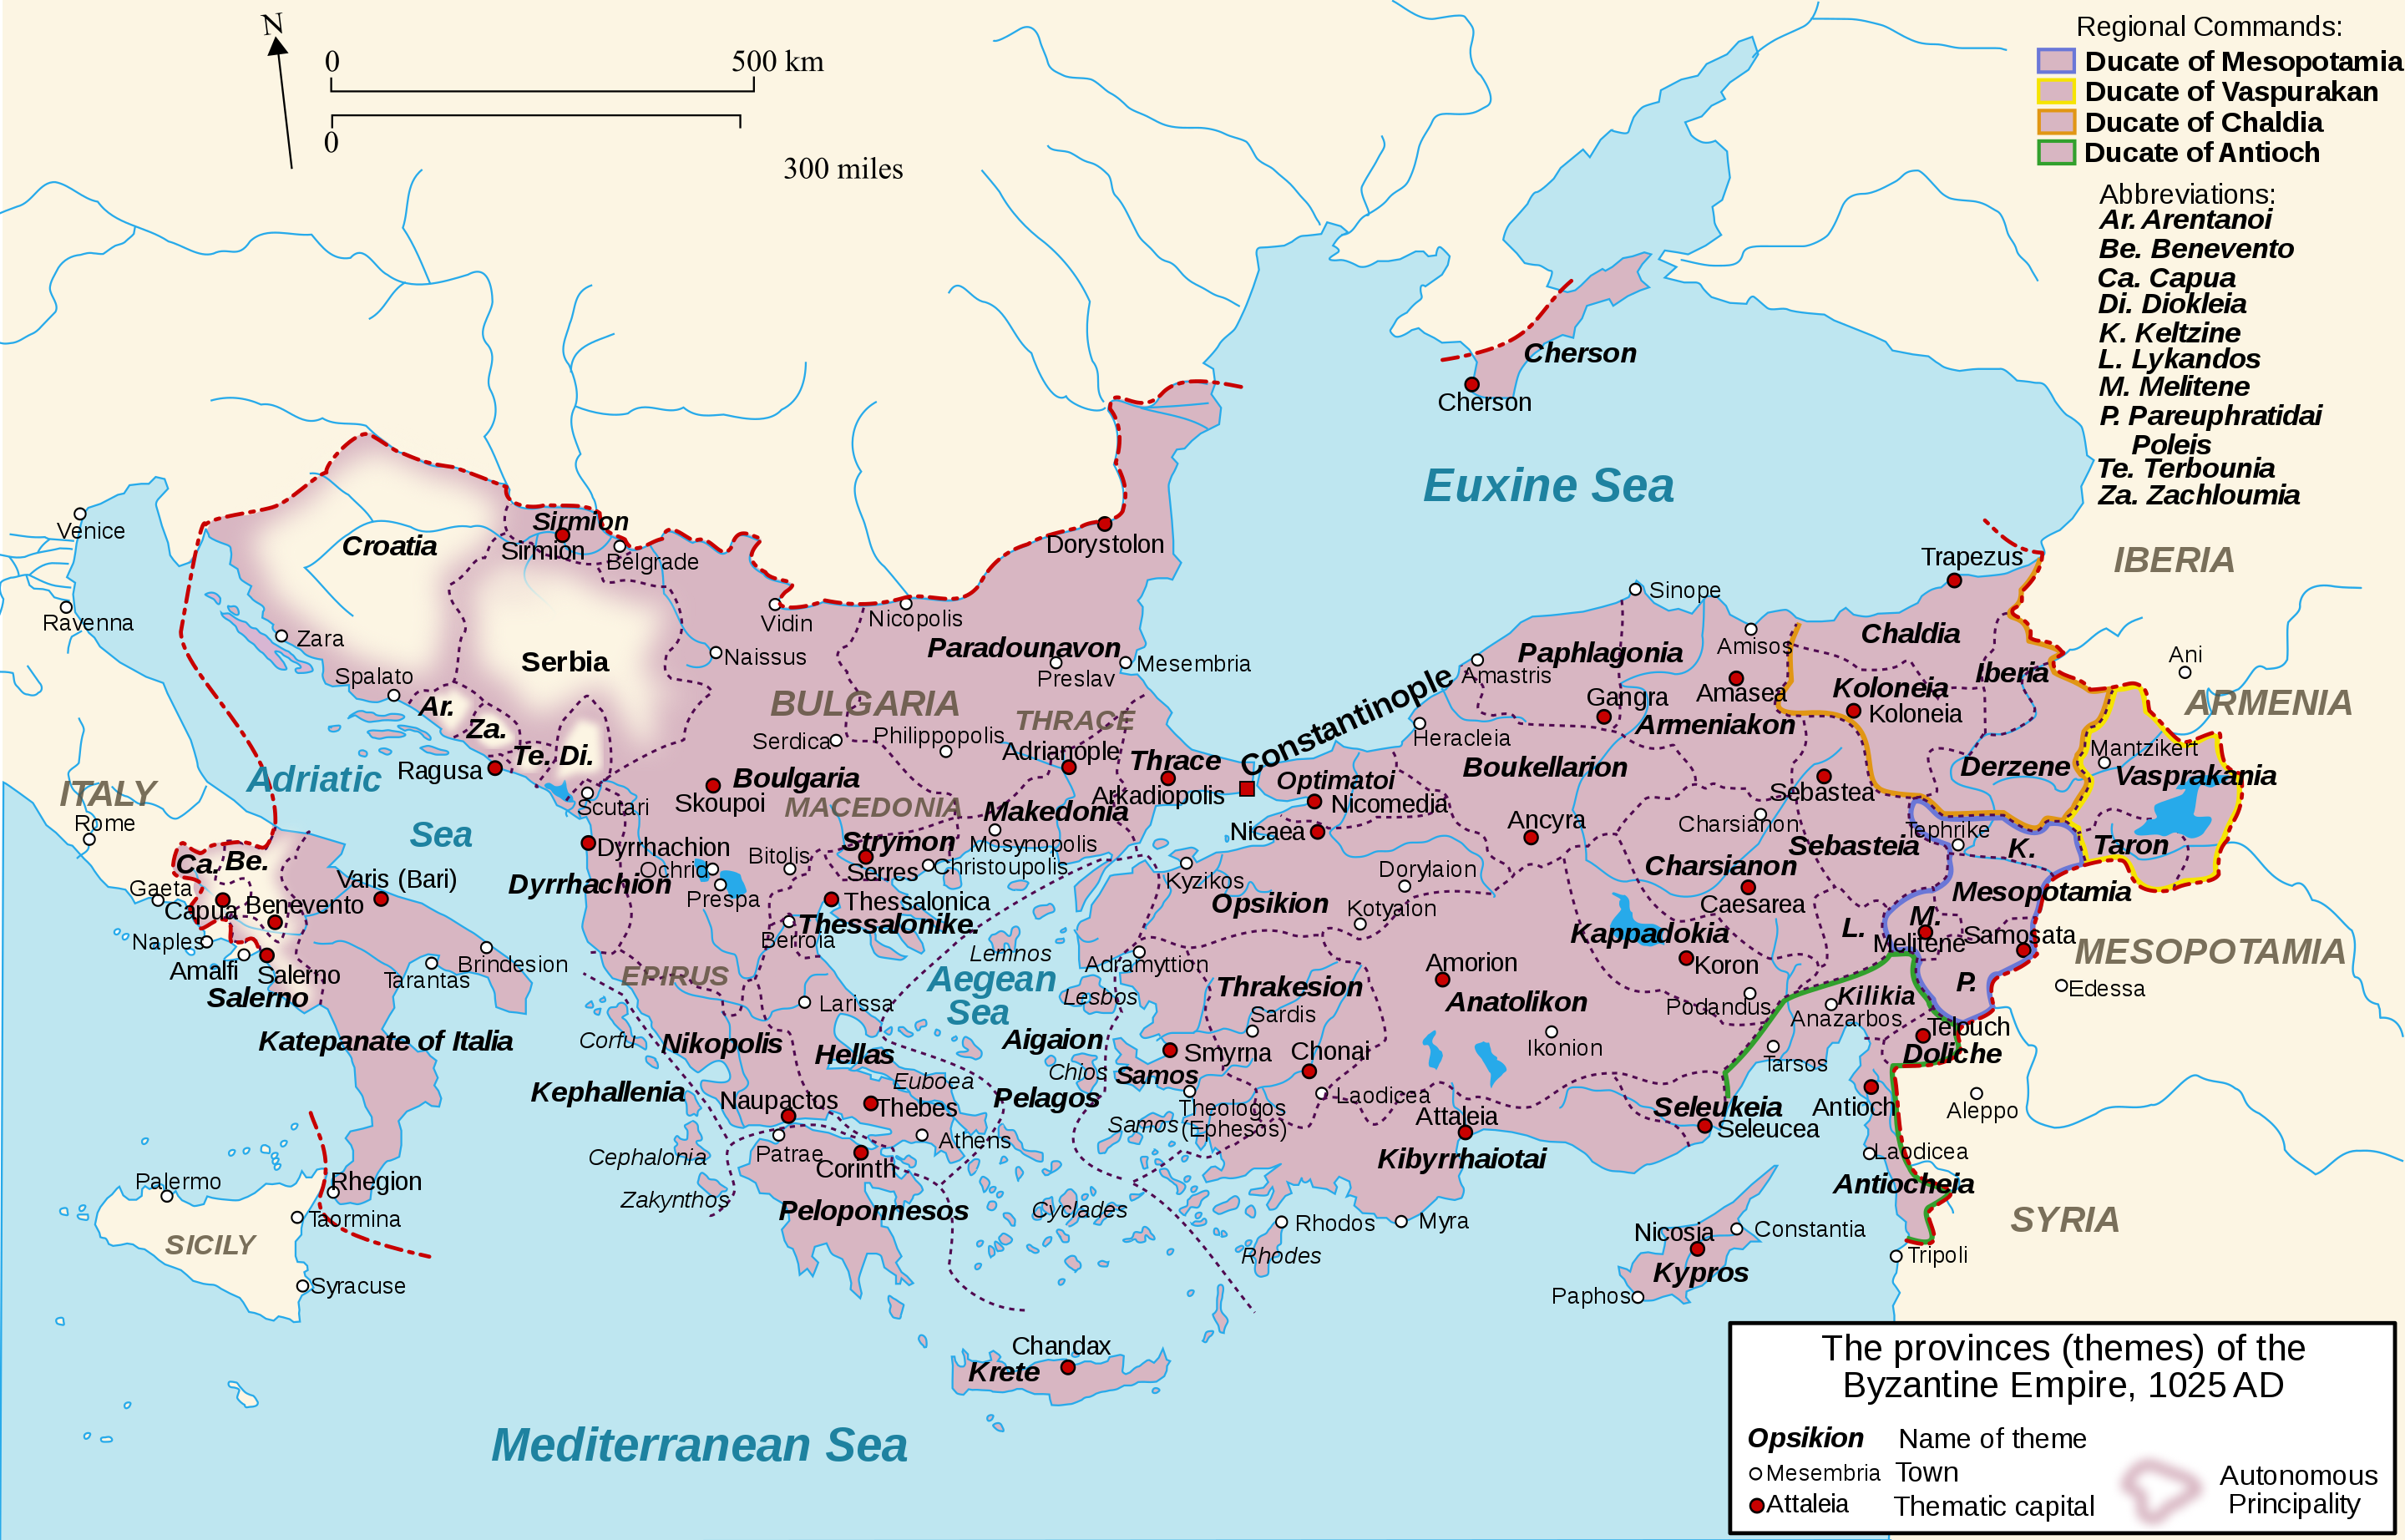
\includegraphics[width=\textwidth]{images/byzantium}
	\end{center}

	Credit: Wikipedia user Cplakidas


\end{frame}

\begin{frame}
	\frametitle{Unreliable, Not Malicious}

	Where this crosses over into the realm of programming is in dealing with the unreliable nature of systems.

	It's not that we think that somewhere out there one of the processes in the system is malicious and trying to make the system fail.

	They have bugs, not ill intent.
\end{frame}


\begin{frame}
	\frametitle{The Dude Abides}
	\begin{center}
		
\includegraphics[width=0.5\textwidth]{images/opinion.jpg}
	\end{center}

	We need a way to deal with the fact that not everyone agrees and sometimes messages get mixed up.

\end{frame}

\begin{frame}
	\frametitle{Organization of the Army}

	There is a \alert{General} who is giving the orders.

	There are also $n$ \alert{Lieutenants} who each are commanding a group of the Empire's troops.

	The individual troops just do what they're told so there's no further concern for their actions.

	The lieutenants can communicate with one another through messages, and they get their orders from the general.

	All of the lieutenants have to work together for their plan to be a success, otherwise there is chaos.
\end{frame}


\begin{frame}
	\frametitle{This is Easy, Right?}

	No problem, you might imagine. The general tells the lieutenants what to do and they do it!

	And if one of the lieutenants does the wrong thing, that lieutenant is a traitor.

	\begin{center}
		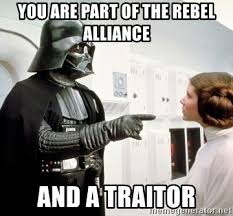
\includegraphics[width=0.4\textwidth]{images/vader-traitor.jpeg}
	\end{center}

	Right?
\end{frame}

\begin{frame}
	\frametitle{Betrayal!}

	But it's not so simple, because the general can be disloyal too.

	Suppose you are a disloyal general.

	Your Emperor has commanded you to attack, but you want the attack to fail, but also seem like it's not your fault.

	What do you do?

\end{frame}

\begin{frame}
	\frametitle{Contradictory Orders It Is}

	You can issue different orders to different lieutenants, they will be all confused and uncoordinated.

	Oh gee darn, I guess the attack didn't go as planned!

	And you can blame the lieutenants who are now dead for going too early, or something.

	It's not like they can defend themselves now...

\end{frame}

\begin{frame}
	\frametitle{Assessing the General's Loyalty}

	A loyal general sends the same message to all lieutenants and a disloyal one sends different messages to different lieutenants.

	It's key to remember that ``loyal'' really means ``functioning'' and ``disloyal'' means ``faulty''.

	It's also worth noting that being in one state or the other is not permanent.

	A functioning unit can be damaged, a malfunctioning one can be repaired, or a problem can be transient.

\end{frame}

\begin{frame}
	\frametitle{How Much Uncertainty?}

	One of the key decisions is about how much disloyalty your system can tolerate.

	Given enough bad actors, things will go wrong. If everyone is disloyal, utter chaos will result.

	But is it enough to tolerate one disloyal participant? Two?

	The line will have to be drawn somewhere...

\end{frame}

\begin{frame}
	\frametitle{Should I Stay or Should I Go Now?}

	In the examples that we will discuss there are two kinds of command: attack and retreat.

	In a real system the options don't have to be quite so binary.

	It is possible that our system produces a tie (no matter how many participants or possible actions we have).

	This usually necessitates a default action be selected.

\end{frame}



\begin{frame}
	\frametitle{Disloyal General, Two Loyal Lieutenants}

	\begin{center}
		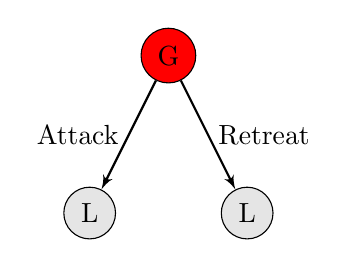
\begin{tikzpicture}
			\node[circle,draw,fill=red, minimum size=0.5] (G) at (0, 0) {G};
			\node[circle,draw,fill=gray!20, minimum size=0.5] (L1) at (-1, -2) {L};
			\node[circle,draw,fill=gray!20, minimum size=0.5] (L2) at (1, -2) {L};
			\draw[-latex', thick] (G) -- (L1) node[midway, left]{Attack};
			\draw[-latex', thick] (G) -- (L2) node[midway, right]{Retreat};
		\end{tikzpicture}
	\end{center}

	Red indicates disloyal; grey indicates loyal.

	What are lieutenants to do?

\end{frame}


\begin{frame}
	\frametitle{He Said What?}

	In the imperfect world of Byzantium the lieutenants can try to figure out if they're about to be mismanaged to literal death by communicating with one another.

	If they are all on the same page then they can do what they're supposed to do; if they're not, then they will fall back on the default option.

	Unfortunately, though, letting the lieutenants communicate is not a complete solution.

\end{frame}


\begin{frame}
	\frametitle{Whose Team Are You On}

	\begin{center}
		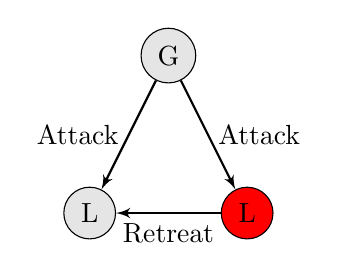
\begin{tikzpicture}
			\node[circle,draw,fill=gray!20, minimum size=0.5] (G) at (0, 0) {G};
			\node[circle,draw,fill=gray!20, minimum size=0.5] (L1) at (-1, -2) {L};
			\node[circle,draw,fill=red, minimum size=0.5] (L2) at (1, -2) {L};
			\draw[-latex', thick] (G) -- (L1) node[midway, left]{Attack};
			\draw[-latex', thick] (G) -- (L2) node[midway, right]{Attack};
			\draw[-latex', thick] (L2) -- (L1) node[midway, below]{Retreat};
		\end{tikzpicture}
	\end{center}

\end{frame}

\begin{frame}
	\frametitle{Do the Math}

	In general if there are $d$ disloyal participants, we will need there to be more than $3d$ participants for the loyal lieutenants to agree on what to do.

	If the general is loyal, then at least $2d$ loyal lieutenants are needed to obey the orders.

	If the general is disloyal then $2d+1$ loyal lieutenants are needed so they can come up with a course of action.

\end{frame}


\begin{frame}
	\frametitle{One Disloyal Participant}

	Imagine that there is at most one disloyal participant.

	If that's the case then all lieutenants should compare notes and decide on the majority course of action.

	Each lieutenant compiles a little table (or array or vector, whatever) of the data received and then decide on what the majority cause of action is.

	It might be simpler to just count the total number of votes, but it would make it harder to figure out later who the traitor is (if there is one).

\end{frame}


\begin{frame}
	\frametitle{Two Disloyal Participants}

	What if we can have two disloyal participants?

	Each lieutenant sending its messages and using a majority-wins vote isn't necessarily going to work here.

	It can happen: the general is disloyal and one of the lieutenants is a collaborator.

	\begin{center}
		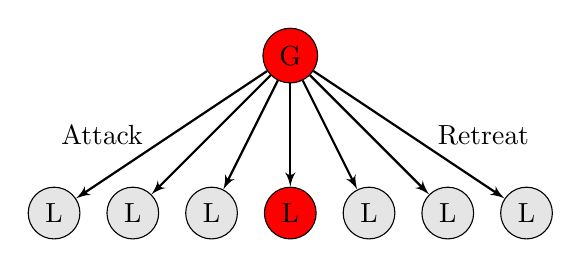
\begin{tikzpicture}
			\node[circle,draw,fill=red, minimum size=0.5] (G) at (0, 0) {G};
			\node[circle,draw,fill=gray!20, minimum size=0.5] (L1) at (-3, -2) {L};
			\node[circle,draw,fill=gray!20, minimum size=0.5] (L2) at (-2, -2) {L};
			\node[circle,draw,fill=gray!20, minimum size=0.5] (L3) at (-1, -2) {L};
			\node[circle,draw,fill=red, minimum size=0.5] (L4) at (0, -2) {L};
			\node[circle,draw,fill=gray!20, minimum size=0.5] (L5) at (1, -2) {L};
			\node[circle,draw,fill=gray!20, minimum size=0.5] (L6) at (2, -2) {L};
			\node[circle,draw,fill=gray!20, minimum size=0.5] (L7) at (3, -2) {L};

			\draw[-latex', thick] (G) -- (L1) node[midway, left]{Attack~~~};
			\draw[-latex', thick] (G) -- (L2);
			\draw[-latex', thick] (G) -- (L3);
			\draw[-latex', thick] (G) -- (L4);
			\draw[-latex', thick] (G) -- (L5);
			\draw[-latex', thick] (G) -- (L6);
			\draw[-latex', thick] (G) -- (L7) node[midway, right]{~~Retreat};
		\end{tikzpicture}
	\end{center}

	What can the collaborating lieutenant do to make sure that the other lieutenants don't come to an agreement?

\end{frame}


\begin{frame}
	\frametitle{Two Disloyal Participants}

	The lieutenants all send one another their instructions.

	The disloyal lieutenant sends one message to half the other participants, and a different message to the other half.

	\begin{center}
		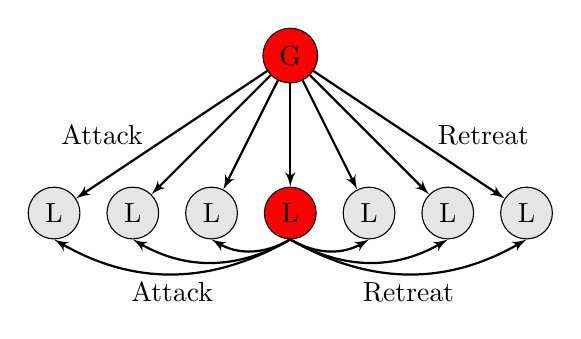
\begin{tikzpicture}
			\node[circle,draw,fill=red, minimum size=0.5] (G) at (0, 0) {G};
			\node[circle,draw,fill=gray!20, minimum size=0.5] (L1) at (-3, -2) {L};
			\node[circle,draw,fill=gray!20, minimum size=0.5] (L2) at (-2, -2) {L};
			\node[circle,draw,fill=gray!20, minimum size=0.5] (L3) at (-1, -2) {L};
			\node[circle,draw,fill=red, minimum size=0.5] (L4) at (0, -2) {L};
			\node[circle,draw,fill=gray!20, minimum size=0.5] (L5) at (1, -2) {L};
			\node[circle,draw,fill=gray!20, minimum size=0.5] (L6) at (2, -2) {L};
			\node[circle,draw,fill=gray!20, minimum size=0.5] (L7) at (3, -2) {L};

			\draw[-latex', thick] (G) -- (L1) node[midway, left]{Attack~~~};
			\draw[-latex', thick] (G) -- (L2);
			\draw[-latex', thick] (G) -- (L3);
			\draw[-latex', thick] (G) -- (L4);
			\draw[-latex', thick] (G) -- (L5);
			\draw[-latex', thick] (G) -- (L6);
			\draw[-latex', thick] (G) -- (L7) node[midway, right]{~~Retreat};
			\draw[-latex', thick] (L4.south) to [bend right] (L7.south);
			\draw[-latex', thick] (L4.south) to [bend right] (L6.south);
			\draw[-latex', thick] (L4.south) to [bend right] (L5.south);
			\draw[-latex', thick] (L4.south) to [bend left] (L3.south);
			\draw[-latex', thick] (L4.south) to [bend left] (L2.south);
			\draw[-latex', thick] (L4.south) to [bend left] (L1.south);

			\node at(-1.5, -3) {Attack};
			\node at(1.5, -3) {Retreat};
		\end{tikzpicture}


	\end{center}
	What do we decide?
\end{frame}

\begin{frame}
	\frametitle{Uh, This Didn't Go Well}
	Half the participants think the majority action is attack and half the participants think the majority action is retreat.

	Summing up what we heard is not sufficient.

	Lieutenants should also talk about what they heard from one another.

	After the general issues instructions, each lieutenant should then communicate with every other to hear what the general said to them.

	Then by reviewing this information, they can decide what to do.

\end{frame}


\begin{frame}
	\frametitle{Double Treason!}

	Consider a simple example where the general is loyal and we have two traitorous lieutenants with a total of seven participants.

	The general issued an order to attack.

	\begin{center}
		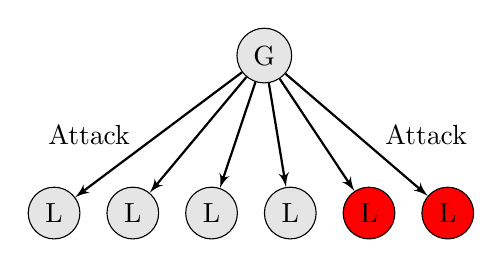
\begin{tikzpicture}
			\node[circle,draw,fill=gray!20, minimum size=0.5] (G) at (-0.33, 0) {G};
			\node[circle,draw,fill=gray!20, minimum size=0.5] (L1) at (-3, -2) {L};
			\node[circle,draw,fill=gray!20, minimum size=0.5] (L2) at (-2, -2) {L};
			\node[circle,draw,fill=gray!20, minimum size=0.5] (L3) at (-1, -2) {L};
			\node[circle,draw,fill=gray!20, minimum size=0.5] (L4) at (0, -2) {L};
			\node[circle,draw,fill=red, minimum size=0.5] (L5) at (1, -2) {L};
			\node[circle,draw,fill=red, minimum size=0.5] (L6) at (2, -2) {L};

			\draw[-latex', thick] (G) -- (L1) node[midway, left]{Attack~~~};
			\draw[-latex', thick] (G) -- (L2);
			\draw[-latex', thick] (G) -- (L3);
			\draw[-latex', thick] (G) -- (L4);
			\draw[-latex', thick] (G) -- (L5);
			\draw[-latex', thick] (G) -- (L6) node[midway, right]{~~Attack};
		\end{tikzpicture}
	\end{center}

\end{frame}

\begin{frame}
	\frametitle{Assemble Your Notes}

	So each lieutenant constructs the following vector.

	The general form is as follows, where $v_{x}$ is the forwarded order we received from lieutenant $x$:

	\begin{center}
		\begin{tabular}{|l|l|l|l|l|l|l|l|}
			\hline
			General & L1      & L2      & L3      & L4      & L5      & L6      \\
			\hline
			?       & $v_{1}$ & $v_{2}$ & $v_{3}$ & $v_{4}$ & $v_{5}$ & $v_{6}$ \\
			\hline
		\end{tabular}
	\end{center}

	So if we are lieutenant 1, we complete the table as below.
	\begin{center}
		\begin{tabular}{|l|l|l|l|l|l|l|l|}
			\hline
			General & L1 & L2 & L3 & L4 & L5 & L6 \\
			\hline
			?       & A  & A  & A  & A  & R  & R  \\
			\hline
		\end{tabular}
	\end{center}

	The value for L1 is what we received from the general, but we get the remaining values from the other lieutenants.

\end{frame}

\begin{frame}
	\frametitle{Compare Notes Again}

	Then the lieutenants just compare notes on this subject as well!

	They send to one another their vectors and assemble them into a table.

	\begin{center}
		\begin{tabular}{|l|l|l|l|l|l|l|l|}
			\hline
			General & L1        & L2        & L3        & L4        & L5        & L6        \\
			\hline
			?       & $v_{1,1}$ & $v_{1,2}$ & $v_{1,3}$ & $v_{1,4}$ & $v_{1,5}$ & $v_{1,6}$ \\\hline
			?       & $v_{2,1}$ & $v_{2,2}$ & $v_{2,3}$ & $v_{2,4}$ & $v_{2,5}$ & $v_{2,6}$ \\\hline
			?       & $v_{3,1}$ & $v_{3,2}$ & $v_{3,3}$ & $v_{3,4}$ & $v_{3,5}$ & $v_{3,6}$ \\\hline
			?       & $v_{4,1}$ & $v_{4,2}$ & $v_{4,3}$ & $v_{4,4}$ & $v_{4,5}$ & $v_{4,6}$ \\\hline
			?       & $v_{5,1}$ & $v_{5,2}$ & $v_{5,3}$ & $v_{5,4}$ & $v_{5,5}$ & $v_{5,6}$ \\\hline
			?       & $v_{6,1}$ & $v_{6,2}$ & $v_{6,3}$ & $v_{6,4}$ & $v_{6,5}$ & $v_{6,6}$ \\\hline
		\end{tabular}
	\end{center}

	In the table each value $v_{i,j}$ is interpreted as ``Lieutenant $i$ says that Lieutenant $j$ reports the general said $v$''.

\end{frame}


\begin{frame}
	\frametitle{I Agree With Myself}

	The entries on the diagonal are redundant because of course each lieutenant agrees with itself.

	Those ``redundant'' entries need to be removed from the table.

	From the point of view of lieutenant 1, let's imagine the table looks like this:
	\begin{center}
		\begin{tabular}{|l|l|l|l|l|l|l|l|}
			\hline
			General & L1 & L2 & L3 & L4 & L5 & L6 \\
			\hline
			?       & ~  & A  & A  & A  & R  & R  \\ \hline
			?       & A  & ~  & A  & A  & R  & R  \\ \hline
			?       & A  & A  & ~  & A  & R  & R  \\ \hline
			?       & A  & A  & A  & ~  & R  & R  \\ \hline
			?       & R  & R  & R  & R  & ~  & R  \\ \hline
			?       & R  & R  & R  & R  & R  & ~  \\ \hline
		\end{tabular}
	\end{center}

\end{frame}

\begin{frame}
	\frametitle{Trust In Yourself}

	Lieutenant 1 does not care what other people THINK they said; so the whole column can be replaced with what was actually said:

	\begin{center}
		\begin{tabular}{|l|l|l|l|l|l|l|l|}
			\hline
			General & L1 & L2 & L3 & L4 & L5 & L6 \\
			\hline
			?       & ~  & A  & A  & A  & R  & R  \\ \hline
			?       & A  & ~  & A  & A  & R  & R  \\ \hline
			?       & A  & A  & ~  & A  & R  & R  \\ \hline
			?       & A  & A  & A  & ~  & R  & R  \\ \hline
			?       & A  & R  & R  & R  & ~  & R  \\ \hline
			?       & A  & R  & R  & R  & R  & ~  \\ \hline
		\end{tabular}
	\end{center}

	Then we'll try to figure out the majority vote for each $j$ in the table.

	So sum up each column:

	\begin{center}
		\begin{tabular}{|l|l|l|l|l|l|l|l|}
			\hline
			General & L1 & L2 & L3 & L4 & L5 & L6 \\
			\hline
			?       & A  & A  & A  & A  & R  & R  \\
			\hline
		\end{tabular}
	\end{center}

\end{frame}


\begin{frame}
	\frametitle{Final Decision}
	4 lieutenants think the general said attack and 2 think the general said retreat.

	The majority wins and the attack proceeds!

	\begin{center}
		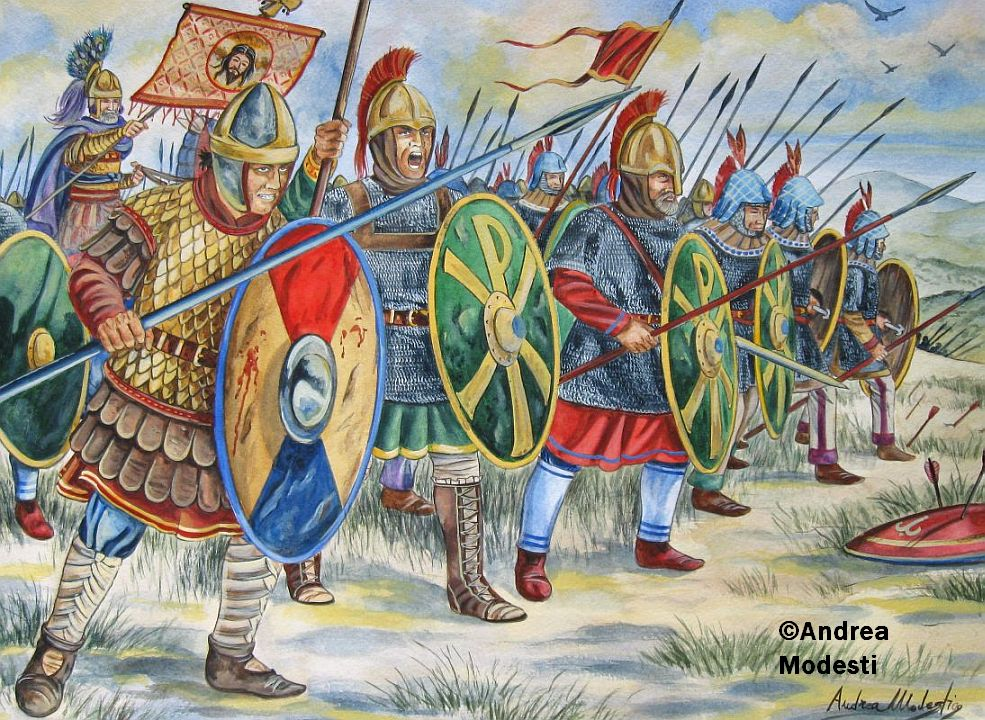
\includegraphics[width=0.6\textwidth]{images/byzantine-army.jpg}
	\end{center}

	Onward to victory, brothers and sisters!

\end{frame}


\begin{frame}
	\frametitle{Or Should I Have Used This One?}

	\begin{center}
		
\includegraphics[width=0.7\textwidth]{images/warhammer.png}
	\end{center}

	This might be less historically accurate, though...

\end{frame}


\begin{frame}
	\frametitle{Mo' Traitors, Mo' Problems}

	If there was one less loyal lieutenant, though, we could have a tie here which would result in picking the default value.

	If the general ordered something other than the default value (e.g., default is retreat and the order was attack) the general will not be happy about this...

\end{frame}

\begin{frame}
	\frametitle{Liar, Liar, Pants on Fire}

	You may have figured out that since disloyal participants can lie at any step of the equation, we can't rely on their data at all.

	That's true!

	In the examples in the course we know that two participants are traitors and I've said they are L5 and L6.

	Therefore we could replace whatever they say with a question mark in the able rather than any particular answer, because they are liars.

	In real life though, \textit{some} message is received -- attack or retreat -- and it's only later we could identify which participants are the traitors.
\end{frame}


\begin{frame}
	\frametitle{We Are Not Amused}

	Remember: we aren't actually interested in determining who the traitors are.


	The goal is just to reach a decision as a group and carry it out.


	\begin{center}
		
\includegraphics[width=0.5\textwidth]{images/hrhqe2.jpg}
	\end{center}


	(In a real-life scenario, of course, things would be different!)

\end{frame}


\begin{frame}
	\frametitle{So, Question Marks}
	
		Back to the example of having eight participants.



	\begin{center}
		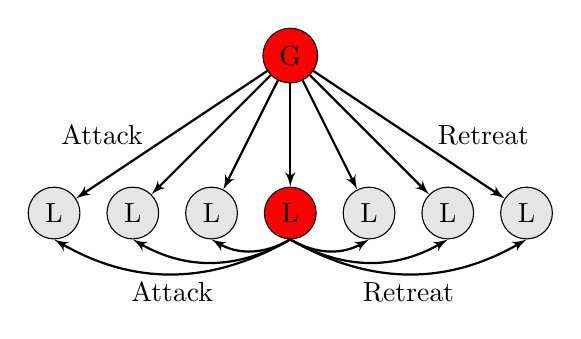
\begin{tikzpicture}
			\node[circle,draw,fill=red, minimum size=0.5] (G) at (0, 0) {G};
			\node[circle,draw,fill=gray!20, minimum size=0.5] (L1) at (-3, -2) {L};
			\node[circle,draw,fill=gray!20, minimum size=0.5] (L2) at (-2, -2) {L};
			\node[circle,draw,fill=gray!20, minimum size=0.5] (L3) at (-1, -2) {L};
			\node[circle,draw,fill=red, minimum size=0.5] (L4) at (0, -2) {L};
			\node[circle,draw,fill=gray!20, minimum size=0.5] (L5) at (1, -2) {L};
			\node[circle,draw,fill=gray!20, minimum size=0.5] (L6) at (2, -2) {L};
			\node[circle,draw,fill=gray!20, minimum size=0.5] (L7) at (3, -2) {L};

			\draw[-latex', thick] (G) -- (L1) node[midway, left]{Attack~~~};
			\draw[-latex', thick] (G) -- (L2);
			\draw[-latex', thick] (G) -- (L3);
			\draw[-latex', thick] (G) -- (L4);
			\draw[-latex', thick] (G) -- (L5);
			\draw[-latex', thick] (G) -- (L6);
			\draw[-latex', thick] (G) -- (L7) node[midway, right]{~~Retreat};
			\draw[-latex', thick] (L4.south) to [bend right] (L7.south);
			\draw[-latex', thick] (L4.south) to [bend right] (L6.south);
			\draw[-latex', thick] (L4.south) to [bend right] (L5.south);
			\draw[-latex', thick] (L4.south) to [bend left] (L3.south);
			\draw[-latex', thick] (L4.south) to [bend left] (L2.south);
			\draw[-latex', thick] (L4.south) to [bend left] (L1.south);

			\node at(-1.5, -3) {Attack};
			\node at(1.5, -3) {Retreat};
		\end{tikzpicture}

	\end{center}

\end{frame}


\begin{frame}
	\frametitle{So, Question Marks}

	Back to the example of having eight participants.

	The value for L1 is what we received from the general, but we get the remaining values from the other lieutenants.

	\begin{center}
		\begin{tabular}{|l|l|l|l|l|l|l|l|}
			\hline
			General & L1 & L2 & L3 & L4 & L5 & L6 & L7 \\
			\hline
			?       & A  & A  & A  & A  & R  & R  & R  \\
			\hline
		\end{tabular}
	\end{center}

	However, if we are lieutenant 7 our vector looks like this instead:

	\begin{center}
		\begin{tabular}{|l|l|l|l|l|l|l|l|}
			\hline
			General & L1 & L2 & L3 & L4 & L5 & L6 & L7 \\
			\hline
			?       & A  & A  & A  & R  & R  & R  & R  \\
			\hline
		\end{tabular}
	\end{center}

\end{frame}

\begin{frame}
	\frametitle{Building the Table}

	From the point of view of lieutenant 1 the table is formed then as follows:

	\begin{center}
		\begin{tabular}{|l|l|l|l|l|l|l|l|}
			\hline
			General & L1 & L2 & L3 & L4 & L5 & L6 & L7 \\
			\hline
			?       & ~  & A  & A  & A  & R  & R  & R  \\ \hline
			?       & A  & ~  & A  & A  & R  & R  & R  \\ \hline
			?       & A  & A  & ~  & A  & R  & R  & R  \\ \hline
			?       & ?  & ?  & ?  & ~  & ?  & ?  & ?  \\ \hline
			?       & A  & A  & A  & R  & ~  & R  & R  \\ \hline
			?       & A  & A  & A  & R  & R  & ~  & R  \\ \hline
			?       & A  & A  & A  & R  & R  & R  & ~  \\ \hline
		\end{tabular}
	\end{center}

	The fourth row is shown as all question marks. Why?

\end{frame}

\begin{frame}
	\frametitle{His Majesty the Emperor Says}
	\begin{center}
		
\includegraphics[width=0.6\textwidth]{images/treason.jpg}
	\end{center}

	Lieutenant 4 is the traitor \& could also lie about what the other lieutenants said.

\end{frame}

\begin{frame}
	\frametitle{Complete the Table and Vector}

	Then replace the first column.

	\begin{center}
		\begin{tabular}{|l|l|l|l|l|l|l|l|}
			\hline
			General & L1 & L2 & L3 & L4 & L5 & L6 & L7 \\
			\hline
			?       & ~  & A  & A  & A  & R  & R  & R  \\ \hline
			?       & A  & ~  & A  & A  & R  & R  & R  \\ \hline
			?       & A  & A  & ~  & A  & R  & R  & R  \\ \hline
			?       & A  & ?  & ?  & ~  & ?  & ?  & ?  \\ \hline
			?       & A  & A  & A  & R  & ~  & R  & R  \\ \hline
			?       & A  & A  & A  & R  & R  & ~  & R  \\ \hline
			?       & A  & A  & A  & R  & R  & R  & ~  \\ \hline
		\end{tabular}
	\end{center}

	Sum up each column:

	\begin{center}
		\begin{tabular}{|l|l|l|l|l|l|l|l|}
			\hline
			General & L1 & L2 & L3 & L4 & L5 & L6 & L7 \\
			\hline
			?       & A  & A  & A  & ?  & R  & R  & R  \\
			\hline
		\end{tabular}
	\end{center}

\end{frame}

\begin{frame}
	\frametitle{It's A Tie...}

	Each of the lieutenants figures out that we have a draw and we then choose the default choice.

	Well, that's grim, but it makes sense: the general issued contradictory orders and the collaborating lieutenant did the same.

	But now instead of half the lieutenants charging in and dying while the others hang back and watch, everyone takes the same action.

	... Even if it's not the one that helps the Empire the most.


\end{frame}

\begin{frame}
	\frametitle{More Traitors!}

	If there three disloyal participants can exist in the system there's another round of data exchange that needs to take place.

	Each lieutenant sends the table formed in the second round to all other lieutenants.

	The more disloyalty there could be in the system, the more rounds the process will go on.

	Communication grows at $n^{2}$ (well, actually worst case $dn^{2}$...)

	So probably we don't tolerate large amounts of treason.

\end{frame}

\begin{frame}
	\frametitle{Trust, But Verify}

	Part of the difficulty comes from the fact that lieutenants can lie about what the general said.

	In the time of Byzantium, wax seals were used (hot wax is poured and then a stamp or ring was used to make an imprint on it).

	In modern times messages can be signed using public-key cryptography.

	Then participants can check whether the received message was genuine.

	An order that does not appear genuine can be disregarded, reducing the ability of disloyal lieutenants to cause confusion.

\end{frame}

\begin{frame}
	\frametitle{Applicability}

	The Byzantine Generals Problem has applicability in all kinds of systems, from space flight to cryptocurrency.

	Whenever we have multiple ``agents'' of some sort that come to their own conclusions about what to do, we can face this issue.

	As long as we know this, we can design our system with this in mind, because pretending it's not going to happen is not a real solution...


\end{frame}



\end{document}

